\documentclass[../main/main.tex]{subfiles}

\begin{document}

\newpage

\chapter{Analysis}
\section{Background}
Mr Myslov is a teacher at Tonbridge School, and currently runs the school chess club. Seldomly, a field day event will be held, in which the club convenes together, playing a chess, or another variant, tournament. This year, Mr Myslov has decided to instead, hold a tournament around another board game, namely laser chess, providing a deviation yet retaining the same familiarity of chess. However, multiple physical sets of laser chess have to be purchased for the entire club to play simultaneously, which is difficult due to it no longer being manufactured. Thus, I have proposed a solution by creating a digital version of the game.

\subsection{Game Description}
Laser Chess is an abstract strategy game played between two opponents. The game differs from regular chess, involving a 10x8 playing board arranged in a predefined condition. The aim of the game is to position your pieces such that your laser beam strikes the opponents Pharoah (the equivalent of a king). Pieces include:

\begin{enumerate}
\item Pharoah
    \begin{itemize}[label=\hyp{}]
    \item Equivalent to the king in chess
    \end{itemize}
\item Scarab
    \begin{itemize}[label=\hyp{}]
    \item 2 for each colour
    \item Contains dual-sided mirrors, capable of reflecting a laser from any direction
    \item Can move into an occupied adjacent square, by swapping positions with the piece on it (even with an opponent’s piece)
    \end{itemize}
\item Pyramid
    \begin{itemize}[label=\hyp{}]
    \item 7 for each colour
    \item Contains a diagonal mirror used to direct the laser
    \item The other 3 out of 4 sides are vulnerable from being hit
    \end{itemize}
\item Anubis
    \begin{itemize}[label=\hyp{}]
    \item 2 for each colour
    \item Large pillar with one mirrored side, vulnerable from the other sides
    \end{itemize}
\item Sphinx
    \begin{itemize}[label=\hyp{}]
    \item 1 for each colour
    \item Piece from which the laser is shot from
    \item Cannot be moved
    \end{itemize}
\end{enumerate}

On each turn, a player may move a piece one square in any direction (similar to the king in regular chess), or rotate a piece clockwise or anticlockwise by 90 degrees. After their move, the laser will automatically be fired. It should be noted that a player’s own pieces can also be hit by their own laser. As in chess, a three-fold repetition results in a draw. Players may also choose to forfeit or offer a draw.

\subsection{Current Solutions}
Current free implementations of laser chess that are playable online are limited, seemingly only available on \url{https://laser-chess.com/}.

\begin{figure}[H]
    \centering
    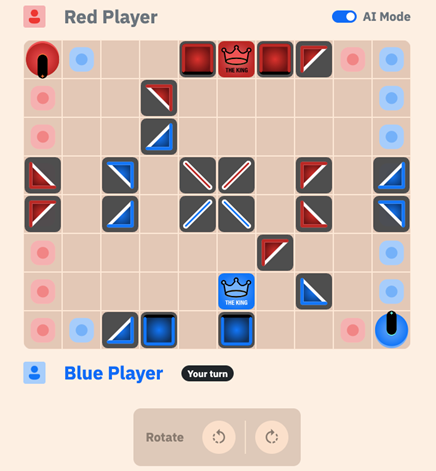
\includegraphics[width=0.6\columnwidth]{../analysis/assets/laser_chess_com.png}
    \caption{Online implementation on \href{https://laser-chess.com/}{laser-chess.com}}
    \label{fig:laser-chess-com}
\end{figure}

The game is hosted online and is responsive and visually appealing, with pieces easy to differentiate and displaying their functionality clearly. It also contains a two-player mode for playing between friends, or an option to play against a functional CPU bot. However, the game lacks the following basic functionalities that makes it unsuitable for my client’s requests:

\begin{itemize}
\item No replay options (going through past moves)
    \begin{itemize}
    \item A feature to look through previous moves is common in digital board game implementations
    \item My client requires this feature as it is an essential tool for learning from past games and to aid in analysing past games
    \end{itemize}
\item No option to save and load previous games
    \begin{itemize}
    \item This QOL feature allows games to be continued on if they cannot be finished in one sitting, and to keep an archive of past games
    \end{itemize}
\item Internet connection required
    \begin{itemize}
    \item My client has specifically requested an offline version as the game will predominantly played in settings where a connection might not be available (i.e. on a plane or the maths dungeons)
    \end{itemize}
\item Unable to change board configuration
    \begin{itemize}
    \item Most versions of laser chess (i.e. Khet) contain different starting board configurations, each offering a different style of play
    \end{itemize}
\end{itemize}
Our design will aim to append the missing feature from this website while learning from their commendable UI design.

\subsection{Client Interview}

\textbf{Q:} Why have you chosen Laser Chess as your request?

\noindent\textbf{A:} Everyone is familiar with chess, so choosing a game that feels similar, and requires the same thinking process and calculations was important to me. Laser chess fit the requirements, but also provides a different experience in that the new way pieces behave have to be learnt and adapted to. It hopefully will be more fun and a better fit for the boys than other variants such as Othello, as the laser aspects and visuals will keep it stimulating.

\bigskip

\noindent\textit{Objectives 1 \& 7}

\noindent Implementing laser chess in a style similar to normal chess will be important. The client also requests for it to be stimulating, requiring both proper gameplay and custom visuals.

\noindent\rule{\textwidth}{0.4pt}

\noindent\textbf{Q:} Have you explored any alternatives?

\noindent\textbf{A:} I remember Laser Chess was pretty popular years ago, but now it’s harder to find a good implementation I can use, since I don’t plan on buying multiple physical copies or paid online copies for every student. I have seen a few free websites offering a decent option, but I’m worried that with the terrible connection in the basement will prove unreliably if everybody tries to connect at once. However, I did find the ease-of-use and simple visuals of some websites pleasing, and something that I wish for in the final product as well.

\bigskip

\noindent\textit{Objective 6}

\noindent The client’s limitations call for a digital implementation that plays offline. Taking inspiration from alternatives, a user-friendly GUI is also expected.

\noindent\rule{\textwidth}{0.4pt}

\noindent\textbf{Q:} What features are you looking for in the final product?

\noindent\textbf{A:} I’m looking for most features chess websites like Chess.com or Lichess offer, a smooth playing experience with no noticeable bugs. I’m also expecting other features such as having a functional timer, being able to draw and resign, as these are important considerations in our everyday chess games too. Since this will be a digital game, I think having handy features such as a indicators for moves and audio cues will also make it more user-friendly and enjoyable. If not for myself, having the option to play against a computer bot will be appreciated as well, since I’ll be able to play during lesson time, or in the case of odd numbers in the tournament. All in all, I’d be happy with a final product that plays Laser Chess, but emulates the playing experience of any chess website well.

\bigskip

\noindent\textit{Objectives 1 \& 3 \& 5}

\noindent Gameplay similar to that of popular chess websites is important to our client, introducing the requirement of subtle features such as move highlighting. A CPU bot is also important to our client, who enjoys thinking deeply and analysing chess games, and so will prove important both as a learning tool and as an opponent.

\noindent\rule{\textwidth}{0.4pt}

\noindent\textbf{Q:} Are there any additional features that might be helpful for your tournament use-cases?

\noindent\textbf{A:} Being able to configure the gameplay will be useful for setting custom time-controls for everybody. I also would like to archive games and share everybody’s matches with the team, so having the functionality to save games, and to go through previous ones, will be highly requested too. Being able to quickly setup board starting positions or share them will also be useful, as this will allow more variety into the tournament and give the stronger players some more interesting options.

\bigskip

\noindent\textit{Objectives 2 \& 4}

\noindent Saving games and customising them is a big logistical priority for a tournament, as this will provide the means to record games and for opponents to all agree on the starting conditions, depending on the circumstances of the tournament.

\section{Objectives}
\subsection{Client Objectives}
The following objectives should be met to satisfy my clients’ requirements:

\begin{enumerate}
\item All laser chess game logic should be properly implemented
    \begin{itemize}
    \item All pieces should be display correct behaviour (i.e reflect the laser correctly)
    \item Option to rotate laser chess pieces should be implemented
    \item Option to move laser chess pieces should be implemented
    \item Game should allocate alternating player’s turns
    \item Travel path of laser should be correctly implemented
    \item Pieces should be automatically detected and eliminated when hit by the laser
    \item Game should automatically detect when a player has lost or won
    \item Three-fold repetition should be automatically detected
    \end{itemize}
\item Save or load game options should be implemented
\label{itm:save-games}
    \begin{itemize}
    \item Games should be encoded into FEN string format
    \item Games can be saved locally into external files
    \item User should be able to scroll through previous games
    \item User should be able to scroll through previous moves
    \item Game should display information relevant to each game, and display moves correctly
    \end{itemize}
\item Other board game requirements should be implemented
    \begin{itemize}
    \item Draws should be made an option
    \item Resigning should be made an option
    \item Timer displaying time left for each player should be displayed
    \item Time logic should be implemented, pausing when it is the opponent’s turn, forfeiting players who run out of time
    \end{itemize}
\item Game settings and config should be customisable
    \begin{itemize}
    \item User should be able to select board colours
    \item User should be able to play against another player or CPU
    \item User should be able to customise timer and duration
    \item User should be able to customise starting board layout and colour
    \end{itemize}
% \item CPU player
%     \begin{itemize}
%     \item CPU player should be functional and display an adequate level of play
%     \item CPU should calculate a move within an adequate timeframe (e.g. 5 seconds)
%     \item CPU should be functional regardless of starting board position
%     \end{itemize}
\item Game UI should improve player experience
    \begin{itemize}
    \item Drag and drop should be implemented
    \item Selected pieces should be clearly marked with an indicator
    \item Indicator showing available squares to move to when clicking on a piece
    \item Destroying a piece should display a visual and audio cue
    \item Captured pieces should be displayed for each player
    \item Status message should display current status of the game (whose turn it is, move a piece, game won etc.)
    \end{itemize}
\item GUI design should be functional and display concise information
    \begin{itemize}
    \item \label{itm:responsive-objective} GUI should always remain responsive throughout the running of the program
    \item Application should be divided into separate sections with their own menus and functionality (e.g. title page, settings)
    \item Navigation buttons (e.g. return to menu) should concisely display their functionality
    \item UI should contain exit and help buttons
    \item UI should be designed for clarity in mind and visually pleasing
    \item Application should be responsive, draggable and resizable
    \end{itemize}
\end{enumerate}

\subsection{Other User Considerations}
Although my current primary client is Mr Myslov, I aim to make my program shareable and accessible, so other parties who would like to try laser chess can access a comprehensive implementation of the game, which currently is not readily available online. Additionally, the code should be concise and well commented, complemented by proper documentation, so other parties can edit and implement additional features such as multiplayer to their own liking.

\section{Research}
Before proceeding with the actual implementation of the game, I will have to conduct research to plan out the fundamental architecture of the game. Reading on available information online, prior research will prevent me from committing unnecessary time to potentially inadequate ideas or code. I will consider the following areas: board representation, CPU techniques and GUI framework.

\subsection{Board Representation}
Board representation is the use of a data structure to represent the state of all pieces on the chessboard, and the state of the game itself, at any moment. It is the foundation on which other aspects such as move generation and the evaluation function are built upon, with different methods of implementation having their own advantages and disadvantages on simplicity, execution efficiency and memory footprint. Every board representation can be classified into two categories: piece-centric or square-centric. Piece-centric representations involve keeping track of all pieces on the board and their associated position. Conversely, square-centric representations track every available square, and if it is empty or occupied by a piece. The following are descriptions of various board representations with their respective pros and cons.

\subsubsection*{Square list}
Square list, a square-centric representation, involves the encoding of each square residing in a separately addressable memory element, usually in the form of an 8x8 two-dimensional array. Each array element would identify which piece, if any, occupies the given square. A common piece encoding could involve using the integers 1 for a pawn, 2 for knight, 3 for bishop, and + and – for white and black respectively (e.g. a white knight would be +2). This representation is easy to understand and implement, and has easy support for multiple chess variants with different board sizes. However, it is computationally inefficient as nested loop commands must be used in frequently called functions, such as finding a piece location. Move generation is also problematic, as each move must be checked to ensure that it does not wrap around the edge of the board.

\subsubsection*{0x88}
0x88, another square\hyp{}centric representation, is an 128\hyp{}byte one\hyp{}dimensional array, equal to the size of two adjacent chessboards. Each square is represented by an integer, with two nibbles used to represent the rank and file of the respective square. For example, the 8\hyp{}integer 0x42 (\lstinline{0100 0010}) would represent the square (4, 2) in zero\hyp{}based numbering. The advantage of 0x88 is that faster bitwise operations are used for computing piece transformations. For example, add 16 to the current square number to move to the square on the row above, or add 1 to move to the next column. Moreover, 0x88 allows for efficient off\hyp{}the\hyp{}board detection. Every valid square number is under 0x88 in hex (\lstinline{0111 0111}), and by performing a bitwise AND operation between the square number and 0x88 (\lstinline{1000 1000}), the destination square can be shown to be invalid if the result is non\hyp{}zero (i.e. contains 1 on 4th or 8th bit).

\subsubsection*{Bitboards}
Bitboards, a piece-centric representation, are finite sets of 64 elements, one bit per square. To represent the game, one bitboard is needed for each piece-type and colour, stored as an array of bitboards as part of a position object. For example, a player could have a bitboard for white pawns, where a positive bit indicates the presence of the pawn. Bitboards are fast to incrementally update, such as flipping bits at the source and destination positions for a moved piece. Moreover, bitmaps representing static information, such as spaces attacked by each piece type, can be pre-calculated, and retrieved with a single memory fetch at a later time. Additionally, bitboards can operate on all squares in parallel using bitwise operations, notably, a 64-bit CPU can perform all operations on a 64-bit bitboard in one cycle. Bitboards are therefore far more execution efficient than other board representations. However, bitboards are memory-intensive and may be sparse, sometimes only containing a single bit in 64. They require more source code, and are problematic for devices with a limited number of process registers or processor instruction cache.

\subsection{CPU techniques}
\subsubsection*{Minimax}
Minimax is a backtracking algorithm that evaluates the best move given a certain depth, assuming optimal play by both players. A game tree of possible moves is formulated, until the leaf node reaches a specified depth. Using a heuristic evaluation function, minimax recursively assigns each node an evaluation based on the following rules:

\begin{itemize}
\item If the node represents a white move, the node’s evaluation is the \textit{maximum} of the evaluation of its children
\item If the node represents a black move, the node’s evaluation is the \textit{minimum} of the evaluation of its children
\end{itemize}

Thus, the algorithm \textit{minimizes} the loss involved when the opponent chooses the move that gives \textit{maximum} loss.

Several additional techniques can be implemented to improve upon minimax. For example, transposition tables are large hash tables storing information about previously reached positions and their evaluation. If the same position is reached via a different sequence of moves, the cached evaluation can be retrieved from the table instead of evaluating each child node, greatly reducing the search space of the game tree. Another, such as alpha-beta pruning can be stacked and applied, which eliminates the need to search large portions of the game tree, thereby significant reducing the computational time.

\subsubsection*{Monte-Carlo Tree Search}
Monte-Carlo Tree Search (MCTS) involves playouts, where games are played to its end by selecting random moves. The result of each playout is then backpropagated up the game tree, updating the weight of nodes visited during the playout, meaning the algorithm successively improves at accurately estimating the values of the most promising moves. MCTS periodically evaluates alternatives to the currently perceived optimal move, and could thereby discover a better, otherwise overlooked, path. Another benefit is that it does not require an explicit evaluation function, as it relies on statistical sampling as opposed to developed theory on the game state. Additionally, MCTS is scalable and may be parallelized, making it suitable for distributed computing or multi-core architectures. However, the rate of tree growth is exponential, requiring huge amounts of memory. In addition, MCTS requires many iterations to be able to reliably decide the most efficient path.

\subsection{GUI framework}
\subsubsection*{Pygame}
Pygame is an open-source Python module geared for game development. It offers abundant yet simple APIs for drawing sprites and game objects on a screen-canvas, managing user input, audio et cetera. It also has good documentation, an extensive community, and receives regular updates through its community edition. Although it has greater customizability in drawing custom bitmap graphics and control over the mainloop, it lacks built-in support for UI elements such as buttons and sliders, requiring custom implementation. Moreover, it is less efficient, using 2D pixel arrays and the RAM instead of utilising the GPU for batch rendering, being single-threaded, and running on an interpreted language.

\subsubsection*{PyQt}
PyQt is the Python binding for Qt, a cross-platform C++ GUI framework. PyQt contains an extensive set of documentation online, complemented by the documentation and forums for its C++ counterpart. Unliked Pygame, PyQt contains many widgets for common UI elements, and support for concurrency within the framework. Another advantage in using PyQt is its development ecosystem, with peripheral applications such as Qt Designer for layouts, QML for user interfaces, and QSS for styling. Although it is not open-source, containing a commercial licensing plan, I have no plans to commercialize the program, and can therefore utilise the open-source license.

\subsubsection*{OpenGL}
Python contains multiple bindings for OpenGL, such as PyOpenGL and ModernGL. Being a widely used standard, OpenGL has the best documentation and support. It also boasts the highest efficiency, designed to be implemented using hardware acceleration through the GPU. However, its main disadvantage is the required complexity compared to the previous frameworks, being primarily a graphical API and not for developing full programs.

\section{Proposed Solution}
\subsection{Language}
The two main options regarding programming language choice, and their pros and cons, are as listed:

\begin{longtable}{ll}
    \toprule
    \multicolumn{2}{c}{Python}\\
    \midrule
    \multicolumn{1}{c}{Pros} & \multicolumn{1}{c}{Cons}\\
    \midrule

    \parbox[t][][t]{0.5\textwidth}{
        \begin{itemize}
            \item Versatile and intuitive, uses simple syntax and dynamic typing
            \item Supports both object-oriented and procedural programming
            \item Rich ecosystem of third-party modules and libraries
            \item Interpreted language, good for portability and easy debugging
        \end{itemize}
    } & \parbox[t][][t]{0.5\textwidth}{
        \begin{itemize}
            \item Slow at runtime
            \item High memory consumption
        \end{itemize}
    }
    \\
    \bottomrule
\end{longtable}

\begin{longtable}{ll}
    \toprule
    \multicolumn{2}{c}{Javascript}\\
    \midrule
    \multicolumn{1}{c}{Pros} & \multicolumn{1}{c}{Cons}\\
    \midrule

    \parbox[t][][t]{0.5\textwidth}{
        \begin{itemize}
            \item Generally faster runtime than Python
            \item Simple, dynamically typed and automatic memory management
            \item Versatile, easy integration with both server-side and front-end
            \item Extensive third-party modules
            \item Also supports object-oriented programming
        \end{itemize}
    } & \parbox[t][][t]{0.5\textwidth}{
        \begin{itemize}
            \item Mainly focused for web development
            \item Comprehensive knowledge of external frameworks (i.e. Electron) needed for developing desktop applications
        \end{itemize}
    }
    \\
    \bottomrule
\end{longtable}

I have chosen Python as the programming language for this project. This is mainly due to its extensive third-party modules and libraries available. Python also provides many different GUI frameworks for desktop applications, whereas options are limited for JavaScript due to its focus on web applications. Moreover, the amount of resources and documentation online will prove invaluable for the development process.

Although Python generally has worse performance than JavaScript, speed and memory efficiency are not primary objectives in my project, and should not affect the final program. Therefore, I have prioritised Python’s simpler syntax over JavaScript’s speed. Being familiar with Python will also allow me to divert more time for development instead of researching new concepts or fixing unfamiliar bugs.

\subsection{Development Environment}
A good development environment improves developer experiences, with features such as auto-indentation and auto-bracket completion for quicker coding. The main development environments under consideration are: Visual Studio Code (VS Code), PyCharm and Sublime Text. I have decided to use VS Code due to its greater library of extensions over Sublime, and its more user-friendly implementation of features such as version control and GitHub integration. Moreover, VS Code contains many handy features that will speed up the development process, such as its built-in debugging features. Although PyCharm is an extensive IDE, its default features can be supplemented by VS Code extensions. Additionally, VS Code is more lightweight and customizable, and contains vast documentation online.

\subsection{Source Control}
A Source Control Tool automates the process of tracking and managing changes in source code. A good source control tool will be essential for my project. It provides the benefits of: protecting the code from human errors (i.e. accidental deletion), enabling easy code experimentation on a clone created through branching from the main project, and by tracking changes through the code history, enabling easier debugging and rollbacks. For my project, I have chosen Git as my version control tool, as it is open-source and provides a more user-friendly interface and documentation over alternatives such as Azure DevOps, and contains sufficient functionality for a small project like mines.

\subsection{Techniques}
I have decided on employing the following techniques, based on the pros and cons outlined in the research section above.

\subsubsection*{Board representation}
I have chosen to use a bitboard representation for my game. The main consideration was computational efficiency, as a smooth playing experience should be ensured regardless of device used. Bitboards allow for parallel bitwise operations, especially as most modern devices nowadays run on 64-bit architecture CPUs. With bitboards being the mainstream implementation, documentation should also be plentiful.

\subsubsection*{CPU techniques}
I have chosen minimax as my searching algorithm. This is due to its relatively simplistic implementation and evaluation accuracy. Additionally, Monte-Carlo Tree Search is computationally intensive, with a high memory requirement and time needed to run with a sufficient number of simulations, which I do not have.

\subsubsection*{GUI framework}
I have chosen Pygame as my main GUI framework. This is due to its increased flexibility, in creating custom art and widgets compared to PyQT’s defined toolset, which is tailored towards building commercial office applications. Although Pygame contains more overhead and boilerplate code to create standard functionality, I believe that the increased control is worth it for a custom game such as laser chess, which requires dynamic rendering of elements such as the laser beam.

I will also integrate Pygame together with ModernGL, using the convenient APIs in for handling user input and sprite drawing, together with the speed of OpenGL to draw shaders and any other effect overlays.

\section{Limitations}
I have agreed with my client that due to the multiple versions of Laser Chess that exist online, together with a lack of regulation, an implementation that adheres to the general rules of Laser Chess, and not strictly to a specific version, is acceptable.

Moreover, due to the time constraints on both my schedules for exams and for the date of the tournament, the game only has to be presented in a functional state, and not polished for release, with extra work such as porting to a wide range of OS systems.

\section{Critical Path Design}
In order to meet my client’s requirement of releasing the game before the next field day, I have given myself a time limit of 12 weeks to develop my game, and have created the following critical path diagram to help me adhere to completing every milestone within the time limit.

\begin{figure}[H]
    \centering
    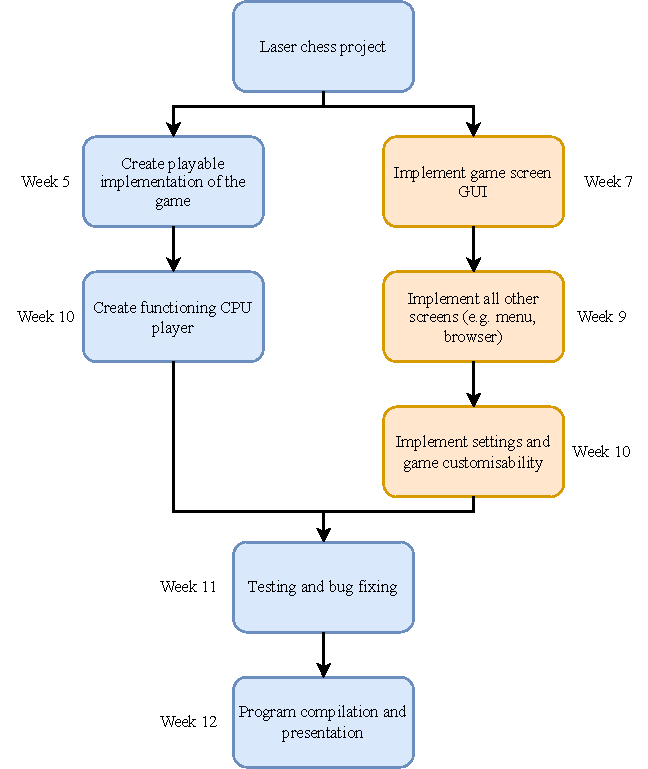
\includegraphics[width=\columnwidth]{../analysis/assets/critical_path_diagram.pdf}
    \label{fig:critical-path-diagram}
\end{figure}

\end{document}